Voxie supports the creation of slices. A slice is a plain intersecting the dataset. 
Its visual representation is defined by all voxel values it intersects.

Voxie supports multiple operations on slices. This includes adjusting, filtering, colorizing and analyzing.

\subsubsection{Creating a slice}

A slice is created by telling the data set (VoxelData) to create a new slice. In the UI this is done by clicking on the \textit{Create Slice} button in the section representing the data set.

After adding a slice a new section will appear displaying the position and rotation of the slice. The 3D image describes the position of the slice within the dataset. Values are coded as x (green),  y (blue), z (red). The rotation is displayed as normalized quaternion.

\begin{figure}[h]
  \centering
  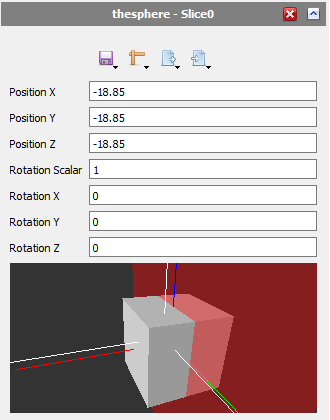
\includegraphics[scale=1.0]{img/2d/3dslice.png}
  \caption{Slice Section}
\end{figure}

\subsubsection{Exporting a slice}

The raw values of the slice can be exported in HDF5 format by clicking on the \textit{Save} button in the slice's section.

\subsubsection{Switching the rotation representation}

The rotation representation of the slice can be switched beteween quaternion or euler angles by clicking on the \textit{rotation representation} button in the slice's section.

\subsubsection{Copy position and rotation}

The position and rotation of the slice can be copy to the system clipbord by clicking on the \textit{copy} button in the slice's section.

\subsubsection{Paste position and/or rotation}

The position and/or the rotation can be paste from the system clipbord to voxie by clicking on the \textit{paste} button and by clicking on the desired option.

\subsubsection{Displaying a slice}

To display a slice Voxie's SliceView plugin has to be used. To add a new Slice View click on Visualizer, then 2D, then Slice.

A dialog will appear. Choosing a slice will create a new window and several new sections.

\begin{figure}[h]
  \centering
  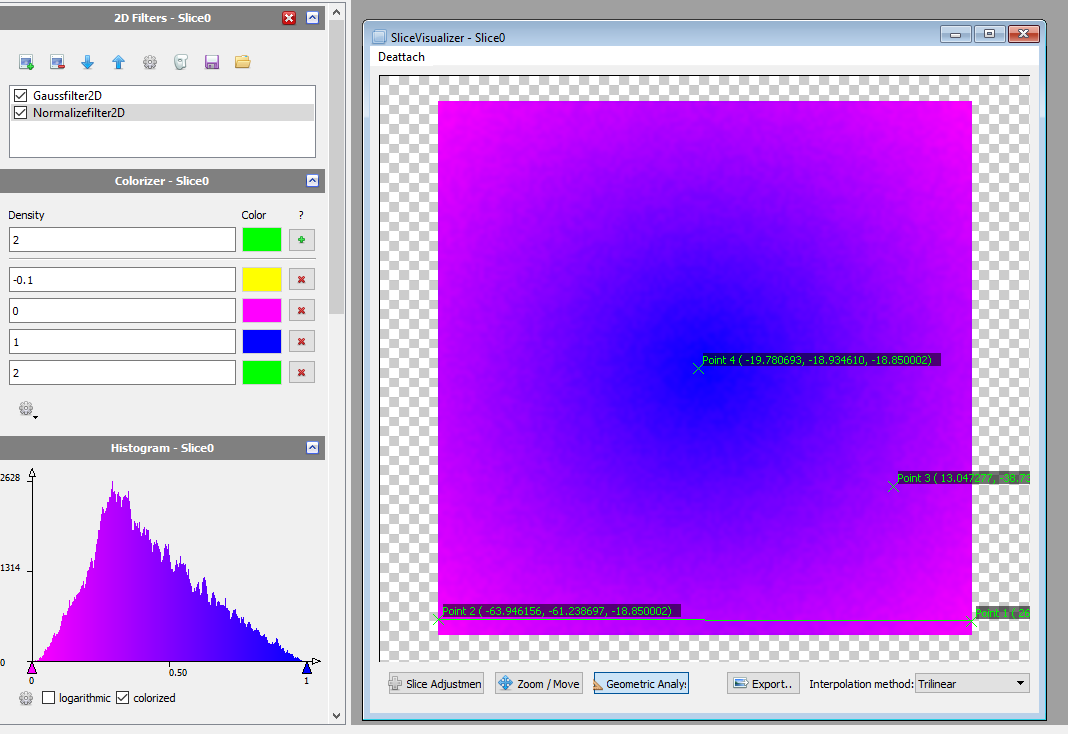
\includegraphics[width=1.0\textwidth]{img/2d/sliceview.png}
  \caption{The Slice View and its sections and tools}
\end{figure}


\subsubsection{The slice view}

By default the slice view window offers a canvas that displays the slice associated with the slice view. It also allows for tools to be used which can modify the slice or display information. Tools can be switched by using the number keys.

\subsubsection{Slice Adjustment Tool}
The slice adjustment tool allows for interactive adjustments to be made to the slices configuration.
When this tool is active the x and y axis of the slice are shown (x = green , y = blue). Notice that x points
right and y points down(!).
\\ \\
The slice's origin can be moved to another point on the plane by [right-clicking]. This is useful because the slice's origin is the pivot point for its rotations.\\
The slice's origin can also be moved along its normal vector with the mouse-wheel or [page-up/down] keys. This
Movement can be fine adjusted by holding down [shift] simultaneously.
\\ \\
The slice's rotation can be adjusted an variuos ways.
To rotate the x-y-plane (rotate arround normal vector) hold down [ctrl] and [drag] the mouse with [left-click] arround the origin. \\
This way you can also rotate arround the other axes. To rotate the slice arround the x axis hold down [ctrl]+[x] and drag with [left-click], with [ctrl]+[y]+[left-click][drag] you can rotate arround the y axis. \\
Alternatively you can use the arrow keys [up]/[down]/[left]/[right] to rotate arround the x or y axis. [shift] can be used to slow down the movement with the arrow keys.
\\ \\
For more arbitrary rotation you can "push down" the slice on a specific point with a simple [left-click]. This causes the slice to tilt towards the direction of clicked point (origin is pivot point). To fully understand this imagine the vector that points from the origin to the click point, the vector that is perpendicular to this vector and the normal vector of the plane is the axis of rotation.\\
The step-size can be reduced by holding down [shift]. 

\subsubsection{Zoom / Move Tool}
The zoom and move tool allows one to zoom and move around the displayed image. Holding the left mouse button and dragging will move the image around. The mouse wheel is used to zoom the image. Toggling the checkbox labeled \textit{Drag redraw?} will allow for less processing power to be required as the image will only be altered when the mouse button is released.

\subsubsection{Geometric Analysis Tool}\label{sec:2dGeometricAnalysis}
The Geometric Analyis allows the user to save points on the slice. This can be done by simply left clicking on the slice. The point will be represented by an x and has its name, as well as its 3d coordinates within the dataset next to it [name (x, y, z)]. Points that were saved are visible in the current image if they are on the slice or within a certain distance in front of or behind it and are colored respectively. Measurements between points (see Geometric Analysis under Sections) are represented by a line between them and - should there be one - the intersection with the slice.

\subsubsection{Interpolation method}
This combobox allows the user to switch between Trilinear and Nearest-neighbor interpolation.\\
Nearest-neighbor is a very simple and fast interpolation option, it simply uses the color of the texel closest to the pixel center for the pixel color. This results in a more blocky image.\\
Trilinear filtering uses linear interpolation to produce a smoother image.


\subsubsection{Mask Selection Tool}
\label{sec:mask}
The Selection Tool allows the User to select an area on the image and on this selected area the filter is applied to. To use this function a filter in the Filter Chain must be selected and only on this filter the mask is applied on. To create a mask you have to click on the mask symbol, then four new buttons appears on the Slice View, \grqq Rectangle\grqq, \grqq Ellipse\grqq, \grqq Polygon\grqq and \grqq Clear\grqq.
\\[12pt]
By clicking on the \textbf{Rectangle Button}, it allows to create a rectangle shape. To do that click and hold the left mouse button and move the mouse. A yellow rectangle appears, this shows the preview of the selection. By realising the left mouse button it finishes the selection and the yellow rectangle turns into red.
\\[12pt]
By clicking on the \textbf{Ellipse Button}, it allows to create a ellipse shape. To do that click and hold the left mouse Button and move the mouse. A yellow ellipse appears, like before it shows the preview of the selection. The first click defines the center of the ellipse. By realising the left mouse button it finishes the selection and the yellow rectangle turns into red.
\\[12pt]
By clicking on the \textbf{Polygon Button}, it allows to create a polygon shape. To do that click on the image, every click is one vertex of the polygon. Every click connects the vertices in yellow, this is just the preview. By pressing space, the polygon shape closes automatically. Notice that at least three vertices are needed to close a polygon shape.
\\[12pt]
By clicking on the \textbf{Clear Button}, it deletes every created shape on the mask only for the selected filter.

\subsubsection{Export Tool}

The export tool will allow for the currently displayed image to be saved. There are three modes available; filtered image, filtered and colorized image or the whole canvas (including borders outside the image).

\subsubsection{Slice View Sections}

A slice view creates six new sections on initialization.

\begin{itemize}
  \item{\emph{2D Filter }\newline This section allows for definition of filters, their order and masks. An ordered set of filters is called a filterchain.}
  \item{\emph{Colorizer}\newline The colorizer section maps values to colors. In between values will be interpolated.}
  \item{\emph{Histogram}\newline The value distribution is visualized here. It also offers advanced options like logarithmic scaling.}
  \item{\emph{Geometric Analysis}\newline This section offers adding measuring points and performing distance measurements between those points.}
  \item{\emph{Grid}\newline This section allows you to place a grid over the slice. It also offers advanced options like change the color of the grid}
  \item{\emph{Ruler}\newline The ruler section gives you the possibility to insert a ruler on the upper and left side. }

\end{itemize}

\begin{figure}[h]
  \centering
  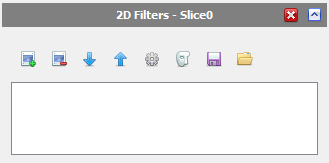
\includegraphics[scale=1.0]{img/2d/2dfilter.png}
  \caption{2D Filter Section}
\end{figure}

\subsubsection{Adding 2D Filters}

A 2D filter can be added by clicking on the \emph{Add Filter} button will open a dialogue allowing one to choose what kind of filter is to be added. Filters are automatically active after creation.

\subsubsection{Removing 2D Filters}

Filters can be removed by highlighting a filter in the section then clicking the \emph{Remove Filter} button.

\subsubsection{Choosing which Filters to apply}

Filters can be temporarily deactivated by toggling the checkbox next to their name.

\subsubsection{Ordering 2D Filters}

Filters are applied in order from top to bottom. Their ordering can be altered by highlighting a filter then pressing the array buttons to move them up or down.

\subsubsection{Configuration of 2D Filters}

Some filters posses a configuration dialogue. The dialogue can be opened by highlighting the desired filter then pressing the \emph{Options} button (\emph{Wheel}).

\subsubsection{Loading and saving Filterchains}

Filterchains including the individual filter settings can be exported and imported using the \emph{Export Filterchain} and \emph{Import Filterchain} buttons. The filterchain will be represented by a human readable xml file.

\subsubsection{Filter Masks}

After activating the filter feature by adding filters, the \emph{Filter Mask} button will activate the filter mask feature in the slice view. This allows for the \emph{Mask Selection Tool} to be used. See \ref{sec:mask} for more information.

\begin{figure}[h]
  \centering
  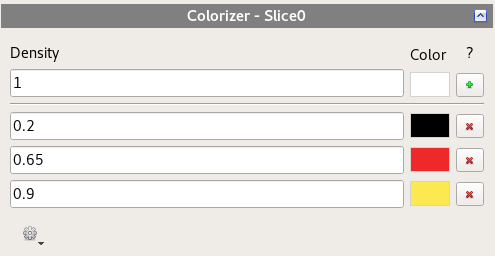
\includegraphics[scale=0.5]{img/2d/colorizer.png}
  \caption{Colorizer Section}
\end{figure}

\subsubsection{Colorizer}\label{sec:Colorizer}

The colorizer maps values to colors. Colors in between the given mappings will be interpolated. A color mapping can be added by pressing the \emph{Add Mapping} button in the first column. This will add a new mapping to the list of mappings below.\newline The colors can be changed by clicking on the displayed color. This will invoke the operating system specific color picker. \newline To remove a mapping simply click on the \emph{Remove Mapping} button. \newline Please note that mappings with the same value will be automatically merged, the new mapping having priority. \newline A click on the gear button opens a small options menu with two options: \emph{Calculate Mapping} automatically calculates a color mapping of two values by using an algorithm based on the whole 3D dataset. \emph{Default mapping} removes the color mapping and replaces it with the default one (0 = black, 1 = white).

\begin{figure}[h!]
  \centering
  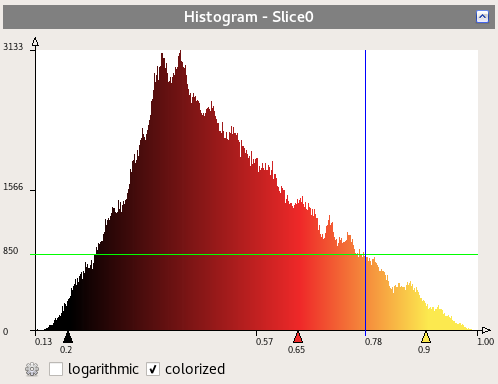
\includegraphics[scale=0.5]{img/2d/histogram}
  \caption{Histogram Section}
\end{figure}  

\begin{figure}[h!]
  \centering
  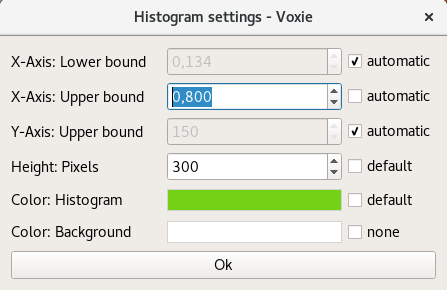
\includegraphics[scale=0.5]{img/2d/histosettings}
  \caption{Histogram Options}
\end{figure}  


\subsubsection{Histogram}

The histogram section shows a visualization of the value distribution of the slice. The scale can be set to linear or logarithmic by switching the \emph{logarithmic} check box. 
\newline The histogram can be colorized dependant on the color mapping values by activating the \emph{colorized} check box. The color mapping (adjusted in the Colorizer) is also permanently shown along the X-Axis as colored triangles.\newline Points within the histogram widget can be marked by a left click with the mouse in the desired area. Move the marker by holding the left mouse button. The related values are shown down the x and y axis. Deleting a marked point works by right clicking with the mouse inside the histogram widget.\newline A gear symbol opens the options dialog. By default, the bouds of the axes are calculated automatically in a way that all values are displayed within the histogram widget. Manual bounds are possible by deactivating the \emph{automatic} checkboxes and setting specific values in the related text boxes. \newline The non-colorized histogram is red by default without a background color. Those color values are adjustable manually by clicking on the colored boxes. \newline The histogram widget can be adjusted in height. This is useful for accurate work.\newline \emph{Hint: All values are applied in real time. Watch the histogram while adjusting the values to get better results}.
 
 \begin{figure}[h!]
  \centering
  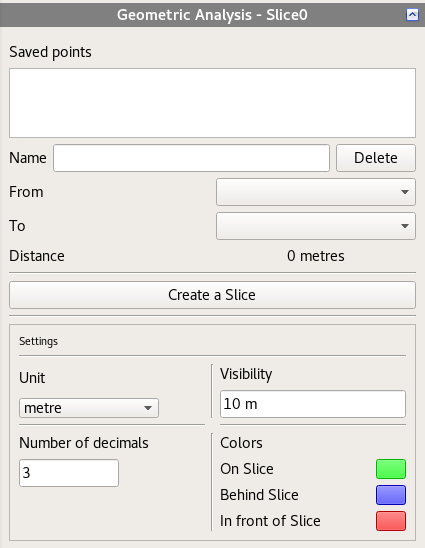
\includegraphics[scale=0.5]{img/2d/geometricAnalysis}
  \caption{Geometric Analysis}
\end{figure}
\subsubsection{Geometric Analysis Section}

This section displays all the saved points in this data set and enables the user to make measurements on them and adjust settings of their representation on the slice image. The "Saved points" box lists all the points currently saved by their name. Having clicked on one, you can change its name by entering a new one in the "Name" field or delete it. Measurements between two points can be made by selecting them from the drop-down menus. The distance between them will then be displayed below and a line will be drawn in the image if they are withtin the range of visibility. 
\newline Clicking "Create a Slice" opens a new window in which you are prompted to choose three points from which either a new slice can be created or the current slice can be moved such that all three points lie upon it. 
\newline In the "Settings" section, you can choose the Unit in which you want distances to be measured as well as the number of decimals to which the measurement should be rounded. It also allows you to change the visual range in front of and behind the slice - i.e. how far points are visible before they fade. Apply changes to those text fields by pressing the "Enter" key. You can also chose the colors of points that are on the slice, behind it or in front of it. Click on the colors to chose a new one.

\begin{figure}[h!]
  \centering
  
\includegraphics[scale=1.0]{img/2d/grid}
  \caption{Grid Section}
\end{figure}

\subsubsection{Grid}

This section allows you to place a grid over the slice. The color, opacity and mesh width can be change via colorpicker, slider and direct text input. In addition, the mode of the grid can be switched. Selectable modes are fixed and automatic. In the fixed mode, the grid has exactly the entered mesh width and does not change. In the automatic mode, on the other hand, the mesh width adjusts so that the grid always remains visible. 

\begin{figure}[h!]
  \centering
  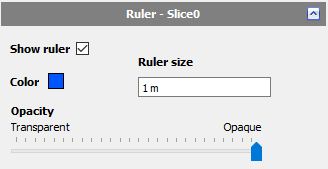
\includegraphics[scale=1.0]{img/2d/ruler}
  \caption{Ruler Section}
\end{figure}  

\subsubsection{Ruler}

This section allows you to place a ruler over the slice. The color, opacity and minimum distance can be change via colorpicker, slider and direct text input. The background of the ruler always takes a complementary color to the selected color of the ruler labeling.
 
\subsubsection{Displaying the difference between two slices}

If two Slices should be compared, the DiffView plugin has to be used. To add a new DIff View click on Visualizer, then 2D, then DiffView.

A dialog will appear. Choosing two slices will create a new window and several new sections.

The DiffView is build similar to the SliceView, thereforce the following subsctions only describe the changes between the DiffView and the SliceView.


\subsubsection{Slice Adjustment Tool}

The Slice Adjustment Tool within the DiffView brings two new buttons: "Switch Slice" to switch the slice that is currently adjusted and "Select Both" to adjust both slices at the same time.

The Origin of the currently not altered Slice will be shown as DashLine. 

\subsubsection{Value Viewer Tool}
The value viewer for the DiffView will always display two values, as there are two Slices, except if the Shift-Key is pressed, then the value for the filtered Image (which is not connected to a slice anymore) will be shown.
